% Options for packages loaded elsewhere
\PassOptionsToPackage{unicode}{hyperref}
\PassOptionsToPackage{hyphens}{url}
%
\documentclass[
]{article}
\usepackage{amsmath,amssymb}
\usepackage{iftex}
\ifPDFTeX
  \usepackage[T1]{fontenc}
  \usepackage[utf8]{inputenc}
  \usepackage{textcomp} % provide euro and other symbols
\else % if luatex or xetex
  \usepackage{unicode-math} % this also loads fontspec
  \defaultfontfeatures{Scale=MatchLowercase}
  \defaultfontfeatures[\rmfamily]{Ligatures=TeX,Scale=1}
\fi
\usepackage{lmodern}
\ifPDFTeX\else
  % xetex/luatex font selection
\fi
% Use upquote if available, for straight quotes in verbatim environments
\IfFileExists{upquote.sty}{\usepackage{upquote}}{}
\IfFileExists{microtype.sty}{% use microtype if available
  \usepackage[]{microtype}
  \UseMicrotypeSet[protrusion]{basicmath} % disable protrusion for tt fonts
}{}
\makeatletter
\@ifundefined{KOMAClassName}{% if non-KOMA class
  \IfFileExists{parskip.sty}{%
    \usepackage{parskip}
  }{% else
    \setlength{\parindent}{0pt}
    \setlength{\parskip}{6pt plus 2pt minus 1pt}}
}{% if KOMA class
  \KOMAoptions{parskip=half}}
\makeatother
\usepackage{xcolor}
\usepackage[margin=1in]{geometry}
\usepackage{color}
\usepackage{fancyvrb}
\newcommand{\VerbBar}{|}
\newcommand{\VERB}{\Verb[commandchars=\\\{\}]}
\DefineVerbatimEnvironment{Highlighting}{Verbatim}{commandchars=\\\{\}}
% Add ',fontsize=\small' for more characters per line
\usepackage{framed}
\definecolor{shadecolor}{RGB}{248,248,248}
\newenvironment{Shaded}{\begin{snugshade}}{\end{snugshade}}
\newcommand{\AlertTok}[1]{\textcolor[rgb]{0.94,0.16,0.16}{#1}}
\newcommand{\AnnotationTok}[1]{\textcolor[rgb]{0.56,0.35,0.01}{\textbf{\textit{#1}}}}
\newcommand{\AttributeTok}[1]{\textcolor[rgb]{0.13,0.29,0.53}{#1}}
\newcommand{\BaseNTok}[1]{\textcolor[rgb]{0.00,0.00,0.81}{#1}}
\newcommand{\BuiltInTok}[1]{#1}
\newcommand{\CharTok}[1]{\textcolor[rgb]{0.31,0.60,0.02}{#1}}
\newcommand{\CommentTok}[1]{\textcolor[rgb]{0.56,0.35,0.01}{\textit{#1}}}
\newcommand{\CommentVarTok}[1]{\textcolor[rgb]{0.56,0.35,0.01}{\textbf{\textit{#1}}}}
\newcommand{\ConstantTok}[1]{\textcolor[rgb]{0.56,0.35,0.01}{#1}}
\newcommand{\ControlFlowTok}[1]{\textcolor[rgb]{0.13,0.29,0.53}{\textbf{#1}}}
\newcommand{\DataTypeTok}[1]{\textcolor[rgb]{0.13,0.29,0.53}{#1}}
\newcommand{\DecValTok}[1]{\textcolor[rgb]{0.00,0.00,0.81}{#1}}
\newcommand{\DocumentationTok}[1]{\textcolor[rgb]{0.56,0.35,0.01}{\textbf{\textit{#1}}}}
\newcommand{\ErrorTok}[1]{\textcolor[rgb]{0.64,0.00,0.00}{\textbf{#1}}}
\newcommand{\ExtensionTok}[1]{#1}
\newcommand{\FloatTok}[1]{\textcolor[rgb]{0.00,0.00,0.81}{#1}}
\newcommand{\FunctionTok}[1]{\textcolor[rgb]{0.13,0.29,0.53}{\textbf{#1}}}
\newcommand{\ImportTok}[1]{#1}
\newcommand{\InformationTok}[1]{\textcolor[rgb]{0.56,0.35,0.01}{\textbf{\textit{#1}}}}
\newcommand{\KeywordTok}[1]{\textcolor[rgb]{0.13,0.29,0.53}{\textbf{#1}}}
\newcommand{\NormalTok}[1]{#1}
\newcommand{\OperatorTok}[1]{\textcolor[rgb]{0.81,0.36,0.00}{\textbf{#1}}}
\newcommand{\OtherTok}[1]{\textcolor[rgb]{0.56,0.35,0.01}{#1}}
\newcommand{\PreprocessorTok}[1]{\textcolor[rgb]{0.56,0.35,0.01}{\textit{#1}}}
\newcommand{\RegionMarkerTok}[1]{#1}
\newcommand{\SpecialCharTok}[1]{\textcolor[rgb]{0.81,0.36,0.00}{\textbf{#1}}}
\newcommand{\SpecialStringTok}[1]{\textcolor[rgb]{0.31,0.60,0.02}{#1}}
\newcommand{\StringTok}[1]{\textcolor[rgb]{0.31,0.60,0.02}{#1}}
\newcommand{\VariableTok}[1]{\textcolor[rgb]{0.00,0.00,0.00}{#1}}
\newcommand{\VerbatimStringTok}[1]{\textcolor[rgb]{0.31,0.60,0.02}{#1}}
\newcommand{\WarningTok}[1]{\textcolor[rgb]{0.56,0.35,0.01}{\textbf{\textit{#1}}}}
\usepackage{graphicx}
\makeatletter
\def\maxwidth{\ifdim\Gin@nat@width>\linewidth\linewidth\else\Gin@nat@width\fi}
\def\maxheight{\ifdim\Gin@nat@height>\textheight\textheight\else\Gin@nat@height\fi}
\makeatother
% Scale images if necessary, so that they will not overflow the page
% margins by default, and it is still possible to overwrite the defaults
% using explicit options in \includegraphics[width, height, ...]{}
\setkeys{Gin}{width=\maxwidth,height=\maxheight,keepaspectratio}
% Set default figure placement to htbp
\makeatletter
\def\fps@figure{htbp}
\makeatother
\setlength{\emergencystretch}{3em} % prevent overfull lines
\providecommand{\tightlist}{%
  \setlength{\itemsep}{0pt}\setlength{\parskip}{0pt}}
\setcounter{secnumdepth}{-\maxdimen} % remove section numbering
\usepackage{booktabs}
\usepackage{caption}
\usepackage{longtable}
\usepackage{colortbl}
\usepackage{array}
\usepackage{anyfontsize}
\usepackage{multirow}
\ifLuaTeX
  \usepackage{selnolig}  % disable illegal ligatures
\fi
\usepackage{bookmark}
\IfFileExists{xurl.sty}{\usepackage{xurl}}{} % add URL line breaks if available
\urlstyle{same}
\hypersetup{
  pdftitle={Assessment},
  hidelinks,
  pdfcreator={LaTeX via pandoc}}

\title{Assessment}
\author{}
\date{\vspace{-2.5em}2024-11-13}

\begin{document}
\maketitle

\subsection{How has COVID-19 impacted respiratory bacterial infections
in
Scotland?}\label{how-has-covid-19-impacted-respiratory-bacterial-infections-in-scotland}

First, I will load the needed library packages.

\begin{Shaded}
\begin{Highlighting}[]
\FunctionTok{library}\NormalTok{(tidyverse)}
\FunctionTok{library}\NormalTok{(janitor) }\CommentTok{\# cleaning data}
\FunctionTok{library}\NormalTok{(gt) }\CommentTok{\# tables}
\FunctionTok{library}\NormalTok{(here) }\CommentTok{\# directory structure}
\FunctionTok{library}\NormalTok{(purrr) }\CommentTok{\# map() function to keep code DRY}
\FunctionTok{library}\NormalTok{(data.table) }\CommentTok{\# Reading multiple CSV files }
\FunctionTok{library}\NormalTok{(glue) }\CommentTok{\# table subtitle}
\FunctionTok{library}\NormalTok{(ggplot2)}
\FunctionTok{library}\NormalTok{(dplyr)}
\FunctionTok{library}\NormalTok{(scales)}
\end{Highlighting}
\end{Shaded}

\subsection{Loading The Data}\label{loading-the-data}

I will be working with data about prescriptions in the community in
Scotland, in specific, prescriptions of the antibiotic Amoxicillin,
which is know known to be prescribed for bacterial respiratory
infections. I will be comparing how presciptions of this antibiotic
differ between Trimethoprim and Metronidazole, two antibiotics which are
prescibed for UTI's and pelvic inflammatory diseases respectively.

The data I will be loading shows all the medicines that have been
dispensed to people by pharmacies in the community. There is a separate
data set for each month, from October 2015. I will be focusing on data
from the month of March as from 2019 to 2024. As march is one of the
peak months for respiratory infections.

The data and the data dictionary can be found here:

\url{https://www.opendata.nhs.scot/dataset/prescriptions-in-the-community}

\begin{Shaded}
\begin{Highlighting}[]
\NormalTok{marchprescriptions }\OtherTok{\textless{}{-}} 
  \FunctionTok{list.files}\NormalTok{(}\AttributeTok{path =} \FunctionTok{here}\NormalTok{(}\StringTok{"marchamoxdata"}\NormalTok{), }\AttributeTok{pattern =} \StringTok{"*.csv"}\NormalTok{, }\AttributeTok{full.names =} \ConstantTok{TRUE}\NormalTok{) }\SpecialCharTok{\%\textgreater{}\%} 
  \FunctionTok{map\_df}\NormalTok{(}\SpecialCharTok{\textasciitilde{}}\FunctionTok{fread}\NormalTok{(.)) }\SpecialCharTok{\%\textgreater{}\%}
  \FunctionTok{clean\_names}\NormalTok{() }\SpecialCharTok{\%\textgreater{}\%} 
  \FunctionTok{mutate}\NormalTok{(}\AttributeTok{hb\_combined =} \FunctionTok{coalesce}\NormalTok{(hbt, hbt2014))}
\end{Highlighting}
\end{Shaded}

\subsection{Visualising the data}\label{visualising-the-data}

I will first explore the data in a table format.

\begin{Shaded}
\begin{Highlighting}[]
\NormalTok{amoxicillin\_data }\OtherTok{\textless{}{-}}\NormalTok{ marchprescriptions }\SpecialCharTok{\%\textgreater{}\%} \CommentTok{\# Create a new object to store the Amoxicillin data.}
  \FunctionTok{filter}\NormalTok{(}\FunctionTok{str\_detect}\NormalTok{(bnf\_item\_description, }\StringTok{"AMOXICILLIN"}\NormalTok{)) }\SpecialCharTok{\%\textgreater{}\%} \CommentTok{\#Filter to only detect and include Amoxicillin data.}
  \FunctionTok{mutate}\NormalTok{(}\AttributeTok{year =} \FunctionTok{substr}\NormalTok{(paid\_date\_month, }\DecValTok{1}\NormalTok{, }\DecValTok{4}\NormalTok{)) }\SpecialCharTok{\%\textgreater{}\%} \CommentTok{\# Remove the \textquotesingle{}03\textquotesingle{} as all the data is from the same month (March).}
  \FunctionTok{group\_by}\NormalTok{(year) }\SpecialCharTok{\%\textgreater{}\%} \CommentTok{\# Group the different types of Amoxicillin prescriptions (tablets, capsules, oral suspensions, etc...) data by year.}
  \FunctionTok{summarise}\NormalTok{(}\AttributeTok{total\_amoxicillin\_march =} \FunctionTok{sum}\NormalTok{(paid\_quantity, }\AttributeTok{na.rm =} \ConstantTok{TRUE}\NormalTok{)) }\CommentTok{\# Summarise the data to show the total amount of Amoxicillin sold in the month of March that year.}

\CommentTok{\# Now we will do the same for Trimethoprim and Metronidazole.}

\NormalTok{trimethoprim\_data }\OtherTok{\textless{}{-}}\NormalTok{ marchprescriptions }\SpecialCharTok{\%\textgreater{}\%} 
  \FunctionTok{filter}\NormalTok{(}\FunctionTok{str\_detect}\NormalTok{(bnf\_item\_description, }\StringTok{"TRIMETHOPRIM"}\NormalTok{)) }\SpecialCharTok{\%\textgreater{}\%} 
  \FunctionTok{mutate}\NormalTok{(}\AttributeTok{year =} \FunctionTok{substr}\NormalTok{(paid\_date\_month, }\DecValTok{1}\NormalTok{, }\DecValTok{4}\NormalTok{)) }\SpecialCharTok{\%\textgreater{}\%}
  \FunctionTok{group\_by}\NormalTok{(year) }\SpecialCharTok{\%\textgreater{}\%} 
  \FunctionTok{summarise}\NormalTok{(}\AttributeTok{total\_trimethoprim\_march =} \FunctionTok{sum}\NormalTok{(paid\_quantity, }\AttributeTok{na.rm =} \ConstantTok{TRUE}\NormalTok{))}

\NormalTok{metronidazole\_data }\OtherTok{\textless{}{-}}\NormalTok{ marchprescriptions }\SpecialCharTok{\%\textgreater{}\%} 
  \FunctionTok{filter}\NormalTok{(}\FunctionTok{str\_detect}\NormalTok{(bnf\_item\_description, }\StringTok{"METRONIDAZOLE"}\NormalTok{)) }\SpecialCharTok{\%\textgreater{}\%} 
  \FunctionTok{mutate}\NormalTok{(}\AttributeTok{year =} \FunctionTok{substr}\NormalTok{(paid\_date\_month, }\DecValTok{1}\NormalTok{, }\DecValTok{4}\NormalTok{)) }\SpecialCharTok{\%\textgreater{}\%}
  \FunctionTok{group\_by}\NormalTok{(year) }\SpecialCharTok{\%\textgreater{}\%} 
  \FunctionTok{summarise}\NormalTok{(}\AttributeTok{total\_metronidazole\_march =} \FunctionTok{sum}\NormalTok{(paid\_quantity, }\AttributeTok{na.rm =} \ConstantTok{TRUE}\NormalTok{))}

\CommentTok{\# Now we will join the data of the three antibiotics to create a table to visualise the data.}

\NormalTok{antibiotics\_table }\OtherTok{\textless{}{-}} \FunctionTok{list}\NormalTok{(amoxicillin\_data, trimethoprim\_data, metronidazole\_data) }\SpecialCharTok{\%\textgreater{}\%} 
  \FunctionTok{reduce}\NormalTok{(full\_join, }\AttributeTok{by =} \StringTok{\textquotesingle{}year\textquotesingle{}}\NormalTok{) }\SpecialCharTok{\%\textgreater{}\%} \CommentTok{\# Join the data by year.}
  \FunctionTok{gt}\NormalTok{() }\SpecialCharTok{\%\textgreater{}\%} \CommentTok{\# Create a table.}
  \FunctionTok{cols\_label}\NormalTok{(}
    \AttributeTok{year =} \StringTok{"Year"}\NormalTok{, }
    \AttributeTok{total\_amoxicillin\_march =} \StringTok{"Amoxicillin"}\NormalTok{,}
    \AttributeTok{total\_trimethoprim\_march =} \StringTok{"Trimethoprim"}\NormalTok{,}
    \AttributeTok{total\_metronidazole\_march =} \StringTok{"Metronidazole"}\NormalTok{) }\SpecialCharTok{\%\textgreater{}\%} \CommentTok{\# Rename the column labels.}
  \FunctionTok{cols\_align}\NormalTok{(}\AttributeTok{align =} \StringTok{"center"}\NormalTok{) }\SpecialCharTok{\%\textgreater{}\%} \CommentTok{\# Center the columns to make it nicer.}
  \FunctionTok{tab\_header}\NormalTok{(}
    \AttributeTok{title =} \StringTok{"Antibiotic Prescriptions in Scotland"}\NormalTok{,}
    \AttributeTok{subtitle =} \StringTok{"During The Month of March"}\NormalTok{) }\SpecialCharTok{\%\textgreater{}\%} \CommentTok{\# Add a title and subtitle.}
  \FunctionTok{fmt\_number}\NormalTok{(}\AttributeTok{columns =} \FunctionTok{c}\NormalTok{(total\_amoxicillin\_march, }
\NormalTok{                         total\_trimethoprim\_march, }
\NormalTok{                         total\_metronidazole\_march),}
             \AttributeTok{decimals =} \DecValTok{0}\NormalTok{, }\AttributeTok{sep\_mark =} \StringTok{","}\NormalTok{) }\SpecialCharTok{\%\textgreater{}\%} \CommentTok{\# Add commas to separate the thousands.}
  \FunctionTok{tab\_style}\NormalTok{(}
    \AttributeTok{style =} \FunctionTok{cell\_text}\NormalTok{(}\AttributeTok{weight =} \StringTok{"bold"}\NormalTok{),}
    \AttributeTok{locations =} \FunctionTok{cells\_title}\NormalTok{(}\AttributeTok{groups =} \StringTok{"title"}\NormalTok{)) }\SpecialCharTok{\%\textgreater{}\%}
  \FunctionTok{tab\_style}\NormalTok{(}
    \AttributeTok{style =} \FunctionTok{cell\_borders}\NormalTok{(}\AttributeTok{sides =} \StringTok{"all"}\NormalTok{, }\AttributeTok{color =} \StringTok{"black"}\NormalTok{, }\AttributeTok{style =} \StringTok{"solid"}\NormalTok{, }\AttributeTok{weight =} \FunctionTok{px}\NormalTok{(}\DecValTok{1}\NormalTok{)),}
    \AttributeTok{locations =} \FunctionTok{list}\NormalTok{(}\FunctionTok{cells\_body}\NormalTok{(), }\FunctionTok{cells\_column\_labels}\NormalTok{())) }\SpecialCharTok{\%\textgreater{}\%}
  \FunctionTok{tab\_style}\NormalTok{(}
    \AttributeTok{style =} \FunctionTok{cell\_fill}\NormalTok{(}\AttributeTok{color =} \StringTok{"lightblue"}\NormalTok{),}
    \AttributeTok{locations =} \FunctionTok{cells\_column\_labels}\NormalTok{()) }\SpecialCharTok{\%\textgreater{}\%}
  \FunctionTok{opt\_table\_outline}\NormalTok{(}\AttributeTok{style =} \StringTok{"solid"}\NormalTok{, }\AttributeTok{width =} \FunctionTok{px}\NormalTok{(}\DecValTok{3}\NormalTok{), }\AttributeTok{color =} \StringTok{"black"}\NormalTok{) }\SpecialCharTok{\%\textgreater{}\%}
  \FunctionTok{opt\_row\_striping}\NormalTok{() }\SpecialCharTok{\%\textgreater{}\%} 
  \FunctionTok{tab\_style\_body}\NormalTok{(}\AttributeTok{style =} \FunctionTok{cell\_fill}\NormalTok{(}\StringTok{"pink"}\NormalTok{), }\AttributeTok{values =} \FunctionTok{c}\NormalTok{(}\DecValTok{1824329}\NormalTok{))}

\NormalTok{antibiotics\_table}
\end{Highlighting}
\end{Shaded}

\begin{table}[!t]
\caption*{
{\large Antibiotic Prescriptions in Scotland} \\ 
{\small During The Month of March}
} 
\fontsize{12.0pt}{14.4pt}\selectfont
\begin{tabular*}{\linewidth}{@{\extracolsep{\fill}}cccc}
\toprule
Year & Amoxicillin & Trimethoprim & Metronidazole \\ 
\midrule\addlinespace[2.5pt]
{2019} & {3,455,623} & {785,254} & {317,228} \\ 
{2020} & {3,528,235} & {779,262} & {276,648} \\ 
{2021} & {\cellcolor[HTML]{FFC0CB}{1,824,329}} & {731,811} & {315,858} \\ 
{2022} & {3,144,001} & {778,682} & {312,013} \\ 
{2023} & {4,617,366} & {756,653} & {315,947} \\ 
{2024} & {4,961,097} & {637,519} & {279,113} \\ 
\bottomrule
\end{tabular*}
\end{table}

I will be looking at the total COVID-19 cases by health boards in
Scotland, the data can be found here:
\url{https://www.opendata.nhs.scot/dataset/viral-respiratory-diseases-including-influenza-and-covid-19-data-in-scotland/resource/2803acc8-8ec3-4c4a-81a5-f10952bf66f4}

\begin{Shaded}
\begin{Highlighting}[]
\NormalTok{weekly\_cases }\OtherTok{\textless{}{-}} \FunctionTok{read.csv}\NormalTok{(}\FunctionTok{here}\NormalTok{(}\StringTok{"weekly\_tests\_cases\_hb\_20241113.csv"}\NormalTok{)) }\SpecialCharTok{\%\textgreater{}\%} 
  \FunctionTok{clean\_names}\NormalTok{()}
\end{Highlighting}
\end{Shaded}

Lets plot the data against each other

\begin{Shaded}
\begin{Highlighting}[]
\NormalTok{covid\_cases }\OtherTok{\textless{}{-}}\NormalTok{ weekly\_cases }\SpecialCharTok{\%\textgreater{}\%} \CommentTok{\#create a new object}
  \FunctionTok{mutate}\NormalTok{(}\AttributeTok{year =} \FunctionTok{substr}\NormalTok{(week\_ending, }\DecValTok{1}\NormalTok{, }\DecValTok{6}\NormalTok{)) }\SpecialCharTok{\%\textgreater{}\%} \CommentTok{\# To extract only the year and the month of march}
  \FunctionTok{filter}\NormalTok{(}\FunctionTok{str\_ends}\NormalTok{(year, }\StringTok{"03"}\NormalTok{)) }\SpecialCharTok{\%\textgreater{}\%}
  \FunctionTok{filter}\NormalTok{(hb }\SpecialCharTok{==} \StringTok{"S92000003"}\NormalTok{) }\SpecialCharTok{\%\textgreater{}\%} \CommentTok{\# Filter to only include the total for all of Scotland (Health Board code S92000003)}
  \FunctionTok{mutate}\NormalTok{(}\AttributeTok{year =} \FunctionTok{substr}\NormalTok{(year, }\DecValTok{1}\NormalTok{, }\DecValTok{4}\NormalTok{)) }\SpecialCharTok{\%\textgreater{}\%}
  \FunctionTok{group\_by}\NormalTok{(year) }\SpecialCharTok{\%\textgreater{}\%} 
  \FunctionTok{summarise}\NormalTok{(}\AttributeTok{covid\_cases =} \FunctionTok{sum}\NormalTok{(weekly\_total\_positive\_tests, }\AttributeTok{na.rm =} \ConstantTok{TRUE}\NormalTok{)) }\SpecialCharTok{\%\textgreater{}\%}
  \FunctionTok{arrange}\NormalTok{(year)}

\NormalTok{joined\_data }\OtherTok{\textless{}{-}} \FunctionTok{list}\NormalTok{(amoxicillin\_data, trimethoprim\_data, metronidazole\_data, covid\_cases) }\SpecialCharTok{\%\textgreater{}\%} 
  \FunctionTok{reduce}\NormalTok{(full\_join, }\AttributeTok{by =} \StringTok{\textquotesingle{}year\textquotesingle{}}\NormalTok{) }\SpecialCharTok{\%\textgreater{}\%} 
  \FunctionTok{mutate}\NormalTok{(}\AttributeTok{year =} \FunctionTok{as.numeric}\NormalTok{(year))}

\NormalTok{line\_plot }\OtherTok{\textless{}{-}}\NormalTok{ joined\_data }\SpecialCharTok{\%\textgreater{}\%} 
  \FunctionTok{ggplot}\NormalTok{(}\FunctionTok{aes}\NormalTok{(}\AttributeTok{x =}\NormalTok{ year)) }\SpecialCharTok{+} 
    \FunctionTok{geom\_point}\NormalTok{(}\FunctionTok{aes}\NormalTok{(}\AttributeTok{y =}\NormalTok{ total\_amoxicillin\_march), }\AttributeTok{colour =} \StringTok{"blue"}\NormalTok{, }\AttributeTok{size =} \DecValTok{2}\NormalTok{) }\SpecialCharTok{+}
    \FunctionTok{geom\_line}\NormalTok{(}\FunctionTok{aes}\NormalTok{(}\AttributeTok{y =}\NormalTok{ total\_amoxicillin\_march), }\AttributeTok{colour =} \StringTok{"blue"}\NormalTok{) }\SpecialCharTok{+}
    \FunctionTok{geom\_point}\NormalTok{(}\FunctionTok{aes}\NormalTok{(}\AttributeTok{y =}\NormalTok{ total\_trimethoprim\_march), }\AttributeTok{colour =} \StringTok{"orange"}\NormalTok{, }\AttributeTok{size =} \DecValTok{2}\NormalTok{) }\SpecialCharTok{+}
    \FunctionTok{geom\_line}\NormalTok{(}\FunctionTok{aes}\NormalTok{(}\AttributeTok{y =}\NormalTok{ total\_trimethoprim\_march), }\AttributeTok{colour =} \StringTok{"orange"}\NormalTok{) }\SpecialCharTok{+}
    \FunctionTok{geom\_point}\NormalTok{(}\FunctionTok{aes}\NormalTok{(}\AttributeTok{y =}\NormalTok{ total\_metronidazole\_march), }\AttributeTok{colour =} \StringTok{"green"}\NormalTok{, }\AttributeTok{size =} \DecValTok{2}\NormalTok{) }\SpecialCharTok{+}
    \FunctionTok{geom\_line}\NormalTok{(}\FunctionTok{aes}\NormalTok{(}\AttributeTok{y =}\NormalTok{ total\_metronidazole\_march), }\AttributeTok{colour =} \StringTok{"green"}\NormalTok{) }\SpecialCharTok{+}
    \FunctionTok{geom\_point}\NormalTok{(}\FunctionTok{aes}\NormalTok{(}\AttributeTok{y =}\NormalTok{ covid\_cases), }\AttributeTok{colour =} \StringTok{"red"}\NormalTok{, }\AttributeTok{size =} \DecValTok{2}\NormalTok{) }\SpecialCharTok{+}
    \FunctionTok{geom\_line}\NormalTok{(}\FunctionTok{aes}\NormalTok{(}\AttributeTok{y =}\NormalTok{ covid\_cases), }\AttributeTok{colour =} \StringTok{"red"}\NormalTok{) }\SpecialCharTok{+}
    \FunctionTok{labs}\NormalTok{(}
        \AttributeTok{title =} \StringTok{"Antibiotic Prescriptions and COVID{-}19 Cases Over Time"}\NormalTok{,}
        \AttributeTok{x =} \StringTok{"Year"}\NormalTok{,}
        \AttributeTok{y =} \StringTok{"Number of Item Prescriptions"}\NormalTok{) }\SpecialCharTok{+}
    \FunctionTok{theme\_minimal}\NormalTok{() }

\NormalTok{line\_plot}
\end{Highlighting}
\end{Shaded}

\begin{verbatim}
## Warning: Removed 1 row containing missing values or values outside the scale range
## (`geom_point()`).
\end{verbatim}

\begin{verbatim}
## Warning: Removed 1 row containing missing values or values outside the scale range
## (`geom_line()`).
\end{verbatim}

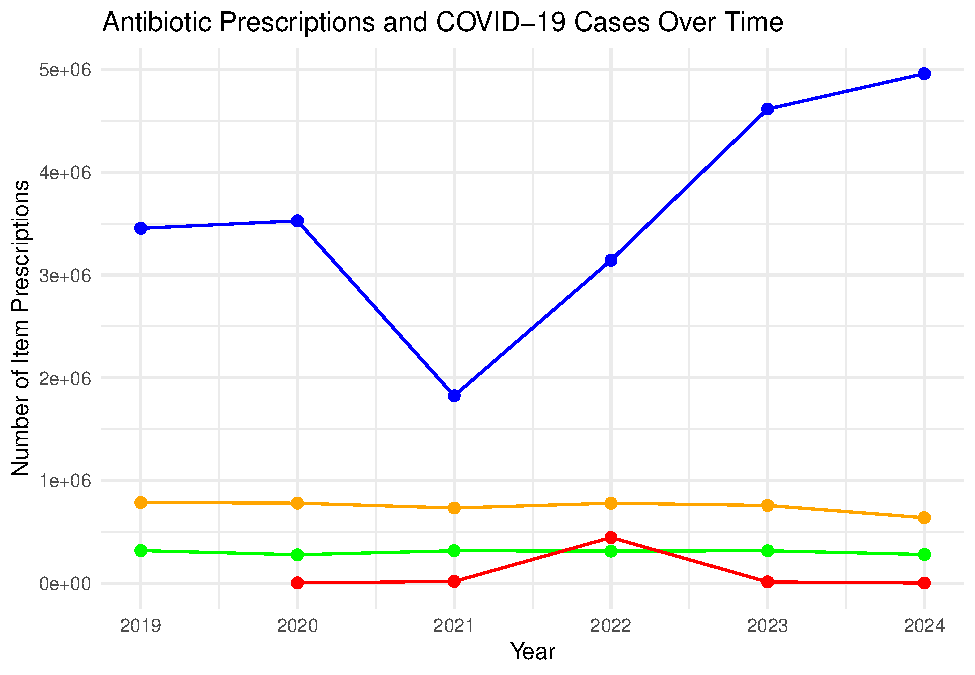
\includegraphics{index_files/figure-latex/unnamed-chunk-1-1.pdf}

\begin{Shaded}
\begin{Highlighting}[]
\NormalTok{amoxicillin\_barplot }\OtherTok{\textless{}{-}}\NormalTok{ joined\_data }\SpecialCharTok{\%\textgreater{}\%}
  \FunctionTok{ggplot}\NormalTok{() }\SpecialCharTok{+}
  \FunctionTok{geom\_bar}\NormalTok{(}\FunctionTok{aes}\NormalTok{(}\AttributeTok{x =}\NormalTok{ year, }\AttributeTok{y =}\NormalTok{ total\_amoxicillin\_march), }\AttributeTok{stat =} \StringTok{"identity"}\NormalTok{, }\AttributeTok{fill =} \StringTok{"pink"}\NormalTok{, }\AttributeTok{colour =} \StringTok{"\#006000"}\NormalTok{) }\SpecialCharTok{+}
  \FunctionTok{geom\_smooth}\NormalTok{(}\FunctionTok{aes}\NormalTok{(}\AttributeTok{x =}\NormalTok{ year, }\AttributeTok{y =}\NormalTok{ covid\_cases }\SpecialCharTok{*} \DecValTok{5}\NormalTok{, }\AttributeTok{group =} \DecValTok{1}\NormalTok{), }\AttributeTok{color =} \StringTok{"red"}\NormalTok{, }\AttributeTok{linewidth =} \DecValTok{1}\NormalTok{) }\SpecialCharTok{+}
  \FunctionTok{labs}\NormalTok{(}
    \AttributeTok{title =} \StringTok{"Scotland Amoxicillin Prescriptions and COVID{-}19 Positive Cases in March"}\NormalTok{,}
    \AttributeTok{x =} \StringTok{"Year"}\NormalTok{, }\AttributeTok{y =} \StringTok{"Amoxicillin (number of items prescribed)"}
\NormalTok{  ) }\SpecialCharTok{+}
  \FunctionTok{scale\_y\_continuous}\NormalTok{(}\AttributeTok{sec.axis =} \FunctionTok{sec\_axis}\NormalTok{(}\SpecialCharTok{\textasciitilde{}}\NormalTok{.}\SpecialCharTok{*}\FloatTok{0.2}\NormalTok{, }\AttributeTok{name =} \StringTok{"COVID{-}19 Positive Cases"}\NormalTok{)) }\SpecialCharTok{+}
  \FunctionTok{theme\_minimal}\NormalTok{()}

\NormalTok{amoxicillin\_barplot}
\end{Highlighting}
\end{Shaded}

\begin{verbatim}
## Warning: Removed 1 row containing non-finite outside the scale range
## (`stat_smooth()`).
\end{verbatim}

\begin{verbatim}
## Warning in simpleLoess(y, x, w, span, degree = degree, parametric = parametric,
## : span too small.  fewer data values than degrees of freedom.
\end{verbatim}

\begin{verbatim}
## Warning in simpleLoess(y, x, w, span, degree = degree, parametric = parametric,
## : pseudoinverse used at 2020
\end{verbatim}

\begin{verbatim}
## Warning in simpleLoess(y, x, w, span, degree = degree, parametric = parametric,
## : neighborhood radius 2.02
\end{verbatim}

\begin{verbatim}
## Warning in simpleLoess(y, x, w, span, degree = degree, parametric = parametric,
## : reciprocal condition number 0
\end{verbatim}

\begin{verbatim}
## Warning in simpleLoess(y, x, w, span, degree = degree, parametric = parametric,
## : There are other near singularities as well. 4.0804
\end{verbatim}

\begin{verbatim}
## Warning in predLoess(object$y, object$x, newx = if (is.null(newdata)) object$x
## else if (is.data.frame(newdata))
## as.matrix(model.frame(delete.response(terms(object)), : span too small.  fewer
## data values than degrees of freedom.
\end{verbatim}

\begin{verbatim}
## Warning in predLoess(object$y, object$x, newx = if (is.null(newdata)) object$x
## else if (is.data.frame(newdata))
## as.matrix(model.frame(delete.response(terms(object)), : pseudoinverse used at
## 2020
\end{verbatim}

\begin{verbatim}
## Warning in predLoess(object$y, object$x, newx = if (is.null(newdata)) object$x
## else if (is.data.frame(newdata))
## as.matrix(model.frame(delete.response(terms(object)), : neighborhood radius
## 2.02
\end{verbatim}

\begin{verbatim}
## Warning in predLoess(object$y, object$x, newx = if (is.null(newdata)) object$x
## else if (is.data.frame(newdata))
## as.matrix(model.frame(delete.response(terms(object)), : reciprocal condition
## number 0
\end{verbatim}

\begin{verbatim}
## Warning in predLoess(object$y, object$x, newx = if (is.null(newdata)) object$x
## else if (is.data.frame(newdata))
## as.matrix(model.frame(delete.response(terms(object)), : There are other near
## singularities as well. 4.0804
\end{verbatim}

\begin{verbatim}
## Warning in max(ids, na.rm = TRUE): no non-missing arguments to max; returning
## -Inf
\end{verbatim}

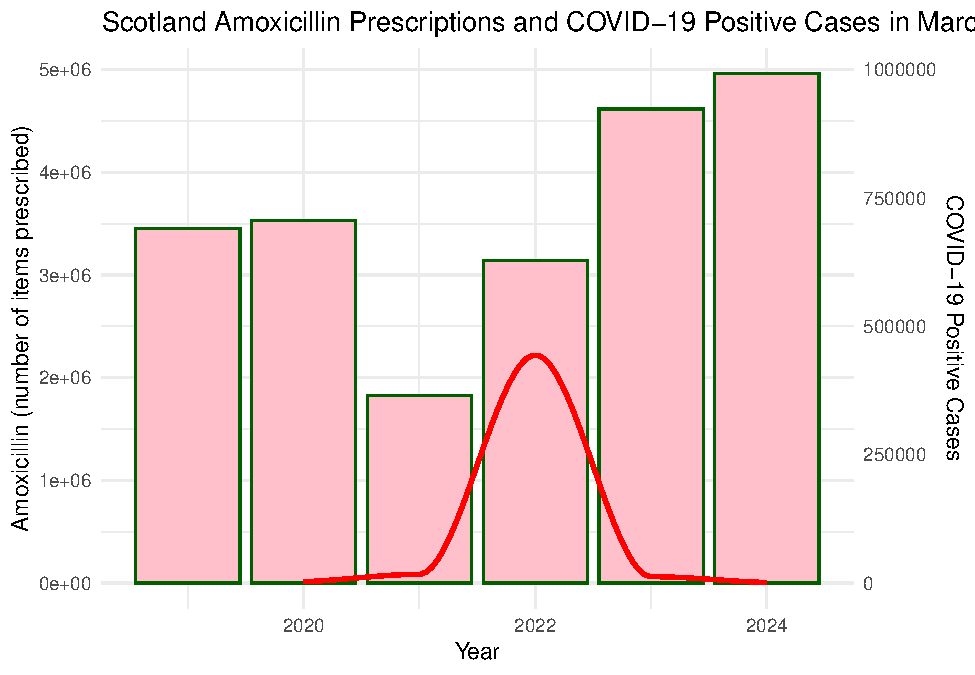
\includegraphics{index_files/figure-latex/unnamed-chunk-1-2.pdf}

\end{document}
